\chapter{Facebook Privacy}
\label{chp:defaultprivacysettings} 


In this chapter we are going to look into the history of Facebook’s privacy settings. We are also going to take a look at how the default privacy settings looks like and map the development of these from 2006 until today. Finally we are going to look at some of the features introduced by Facebook over the years, and how these features have effected peoples privacy. 

\section{Privacy on Facebook}\label{sec:privacy_on_facebook}

-dra inn undersøkelse 
-hva slags type settings som finnes? 


\section{Default Privacy Settings on Facebook}\label{sec:default_privacy_settings}

\paragraph{}
Facebook has evolved from being a networking site for students attending Harvard to becoming a global phenomenon. Facebook's user interface has gone through several changes over the years, which has brought both joy and frustration to the users. When these changes have been made, there has also been adjustments to the default privacy settings as well \cite{EvoPriv2}. At the beginning, in 2005, when Facebook first was applied outside of Harvard University, the users personal information was only accessible to a users Facebook friends and to people connected to the same network on Facebook \cite{EvoPriv}. 

The main changes to the default privacy settings are emphasized in \tref{tab:dps}. 

\begin{center}
\begin{table}
\caption{\label{tab:dps}Changes in the default privacy settings on Facebook from 2005 until today. \cite{EvoPriv,PrivTimeline}}
    \begin{tabular}{ | l | p{9cm} |}
    \hline
    \textbf{Year} & \textbf{Default Privacy Settings} \\ 
    \hline
    2005 & Personal information (e.g., name and profile picture) is 	only visible to specific groups specified in your privacy 			settings.\\ 
    \hline
    2006 & The only information displayed in your profile is your 		school and specified local area. \\ 
    \hline
    2007 & Name, name of school (network) and profile picture 			(thumbnail) is available to all Facebook users.\\
    \hline
    November 2009 & Name, profile picture and demographics is 			available and searchable to the entire Internet. In addition to 	this, list of friends are visible to all Facebook users.\\
	\hline
    December 2009 & Your name, profile picture, list of friends, 		pages you are fan of, demographics and likes are available for 		the entire Internet.\\
    \hline
    April 2010 & The entire Internet can see everything, except 		wall posts that are limited to friends and photos that are 			limited to your network. \\
    \hline
    2011 &  \\
    \hline
    2012 & \\
    \hline
    November 2013 & The entire Internet can see everything, except posts you've been tagged in on your timeline and others posts on your timeline, which are limited to friends of friends. \\ 
    \hline
    \end{tabular}
   \end{table}
\end{center}


\paragraph{}
Zuckerberg said this in a one of his meetings; “I mean, one way to look at the goal of the site is to increase people’s understanding of the world around them, to increase their information supply,” he said. “The way you do that best is by having people share as much information as they are comfortable with. The way you make people comfortable is by giving them control over exactly who can see what” \cite{MeMedia}.


\paragraph{}
User control became a hot topic i 2006. There had been reported that sex- offenders was using social networks to pick out their victims. MySpace found out that several teenagers had been assaulted by people they meet at the site. Facebook also received some negative mention in the press. Numerous times the campus police had to shut down big parties announced on Facebook. In 2005 a student a Fisher college was expelled after posting this comment about the schools police officer "needs to be eliminated" \cite{MeMedia}.  
In general the privacy settings and restrictions that Facebook has have protected the users. They can easily change the setting and decide who can see what.

“I think that understanding that there might not be any difference between what people are doing online and offline is something really important,” Zuckerberg said firmly. “People are online because it is a more efficient way of doing things.” A man in the audience asked Zuckerberg about some pictures of students drinking at an East Coast college, which, he claimed, had appeared on Facebook and had led to the expulsion of several students. “First of all, it’s pretty stupid if you put up pictures of you doing drugs on Facebook,” Zuckerberg said. “I think that that’s just sort of the deviant behavior on the very far end of the distribution. . . . I bet that those kids do not post pictures of them doing drugs on Facebook anymore.” He went on, “Obviously that’s a pretty shitty way to learn that, like, you’re not supposed to post pictures like that on Facebook, but, I mean, the fact that everyone here hears this and is kind of shocked means that more than just those few people learn from that mistake, right? And the system is going to reach an equilibrium that makes sense” \cite{MeMedia}.

\paragraph{}
"Somehow we missed this point with News Feed and Mini-Feed and we didn't build in the proper privacy controls right away. This was a big mistake on our part, and I'm sorry for it." \cite{FacebookStoryInceptionToIsp}

\paragraph{}
Mark Zuckerberg wrote this in a letter to possible investors \cite{LetterToInvestors};

\textit{Facebook was not originally created to be a company. It was built to accomplish a social mission - to make the world more open and connected.}

\textit{People sharing more - even if just with their close friends or families - creates a more open culture and leads to a better understanding of the lives and perspectives of others. We believe that this creates a greater number of stronger relationships between people, and that it helps people get exposed to a greater number of diverse perspectives.}

\textit{By helping people form these connections, we hope to rewire the way people spread and consume information. We think the world's information infrastructure should resemble the social graph - a network built from the bottom up or peer-to-peer, rather than the monolithic, top-down structure that has existed to date. We also believe that giving people control over what they share is a fundamental principle of this rewiring.}

\textit{We think a more open and connected world will help create a stronger economy with more authentic businesses that build better products and services.}


\subsection{Default settings for teens}
Each time a user on Facebook share a status update, the user chooses who the post is visible to, see \fref{fig:newPost}. The change you make will remain the same in future posts, unless you decide to change it. Up until today the default audience is set to "public", but for teens between 13-17 years, it has been "friends of friends". On October 16th Facebook announced to change the default setting for teens \cite{defaultTeens}. Now the initial audience for posts are "friends". Teens can later change this to "public", this was not a option before. Teens are active users of social media, and have want to be heard, either it is political engagement or an opinion on a movie. Further Facebook allows teens to turn on Follow, by doing this their public posts will show up in people's news feeds. Facebook designed these changes to improve the facebook experience for young people. In \cite{defaultTeens} Facebook also makes it clear that they take the safety of teens very seriously, and therefore have created a more extensive warning message, shown in  \fref{fig:teensSharePost}. This message appears when a teen changes the audience for their post. If they continue to post to the public, they will will get an additional reminder message, as shown in  \fref{fig:sharePost}.

\begin{figure}[h!]
\centering
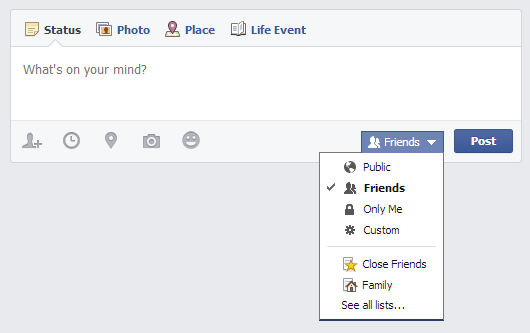
\includegraphics[width=0.8\textwidth]{new_post.png}
\caption{Choosing who can see the status update.} 
\label{fig:newPost}
\end{figure}

\begin{figure}[h!]
\centering
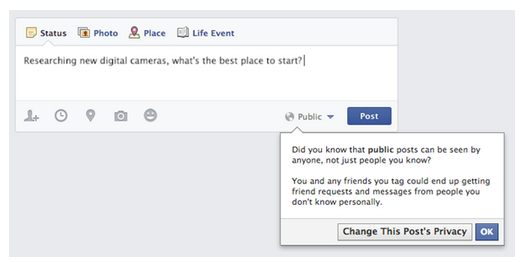
\includegraphics[width=0.8\textwidth]{teensSharePost.png}
\caption{The message that is shown to a teens when posting to the public \cite{defaultTeens}.} 
\label{fig:teensSharePost}
\end{figure}

\begin{figure}[h!]
\centering
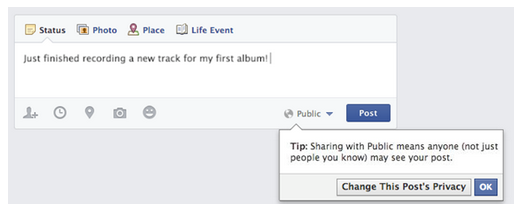
\includegraphics[width=0.8\textwidth]{sharePost.png}
\caption{The message that is shown to a regular user when posting to the public \cite{defaultTeens}.} 
\label{fig:sharePost}
\end{figure}

\section{Facebook Features - Impact on your Privacy}\label{sec:facebook_features}

\subsection{Beacon}
-Det må fylles ut mer her!

\paragraph{}
At the end of 2007 Facebook lauched the feature called Beacon. Beacon was created to help users easily share their information with their friends. Beacon was part of and advertisement system that Facebook used. It tracked peoples activity on the web and made it possible for users to share this with their friends. When Beacon was launched it had 44 partner sites, and these sites had the possibility to post a users activity on the user's newsfeed \cite{BeaconWebsites}. Beacon was a sentral element in Facebook's ad system created to connect businesses with users, and making it easier for the businesses to target the advertising. 

\paragraph{}
In a blog post, Mark Zuckerberg apologized for the way the feature was created and for the handling of the complaints in hindsight. 
\cite{Beacon} 


\subsection{Graph search}


\subsection{Facebook removes search privacy setting}
Facebook announced October 11 that they will remove the setting that has made it possible for Facebooks users to hide from the ability to be looked up on the Internet\cite{searchSetting}. It was only the users that have not used the setting "who can look up my timeline by name" in December by last year that was affected by the change. Facebook explains the removal of the feature by it being outdated, and that there are several others ways to find a persons time line. They argue that it can be confusing for the user when they try to look up someone and do not find them. Mark Zuckerberg said that a users should do things they want to keep secret.

(sånn jeg ser det så er det jo fult mulig å søke opp hvem som helt på faceboko sin egen søkefunksjon, det betyr jo ikke ta jeg ønsker å være søkbar på google. 

\subsection{Timeline}
As mentioned in section \ref{sec:facebookhistory} in Chapter 1, the Facebook timeline was introduced in December 2011 \cite{EvolutionOfFacebook}. This feature made the entire history of the users visible: your posts, posts by others, likes, photos, links, pages liked, comments and other things that you have shared on Facebook. The timeline showed much more than the old profile did, and it was far more visual \cite{timeline}. On the top of your timeline it is room for a big photo. This photo is called a \emph{cover photo}. Cover photos are publicly available, and it is not possible to change the settings for them. You can of course choose which photo you want as your cover photo, or just choose not to have a photo there at all. When scrolling down your timeline , you'll see photos, posts etc. and different events in your life in order of when they happend in time \cite{timeline}. You can look at it as the story of your life. You get the opportunity to "go back in time" and fill in the blanks. If you want to emphasize, for example an event or a photo, you can highlight it with a star, or on the other hand, if you want to hide something from the timeline you can also do so. 

\paragraph{Privacy concerns regarding Facebook timeline}
When timeline was introduced many people became overwhelmed by the changes, and felt they lost control over their privacy. When you agreed to start using timeline, you got a certain period of time to review and edit your timeline before making it public. This gave the users the opportunity to clean up their timeline before everyone else could view the content of it. Cleaning up the timeline can be done using something called the "Activity Log" \cite{activitylog}, which is shown in \fref{fig:activitylog}. The activity log is basically a list over everything ever done in connection with you on Facebook, either done by you or by others. The activity log also makes it easy to view and change the audience for the different "activities". If you are an active user of Facebook, reviewing the whole activity log can be very time consuming. 

\begin{figure}[h!]
\centering
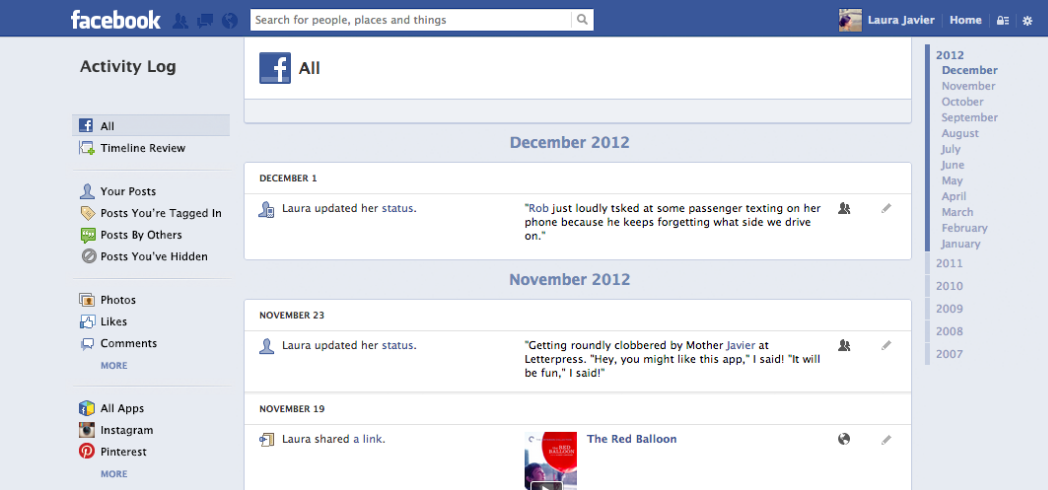
\includegraphics[width=1\textwidth]{activity_log.png}
\caption{Example of an activity log on Facebook. On the left side you see types of content. If you want to view for example "Posts by others" you can do so by clicking on it. To the right you see a list of the years and months. You can click on which year or month you want, and review the activity from that year/month \cite{activitylog}} 
\label{fig:activitylog}
\end{figure}


\paragraph{}
The introduction of timeline was not in itself a privacy breach since you had, and still have, the opportunity to decide what should be visible on it, and what should be hidden. On the other hand, there are people who are extra exposed when Facebook introduced new major changes, like the timeline. Lets refer back to section \ref{sec:relatedwork_facebookprivacy} in Chapter \ref{chp:relatedwork}, where we highlighted some of the findings from the survey addressed in the paper "Facebook privacy settings; Who cares?" by danah boyd and Eszter Hargittai \cite{whocares}. boyd and Hargittai concluded their paper, based on their survey and findings, that experience and Internet skill is important to take into account in regard to how people handle their privacy settings on Facebook. Since familiarity with technology plays a role in how people handle their Facebook privacy settings, one can assume that the least skilled people get more exposed when Facebook changes the outline of the default privacy settings. 
This can be seen in the context with the introduction of the timeline. The least skilled users of Facebook that perhaps do not know how to change their privacy settings, probably was left extra exposed when the timeline was introduced and their timeline may have shown, and may still show, more than they actually would prefer. 


There also exits privacy settings connected to you timeline under "Timeline and tagging" in your settings on Facebook. You can regulate who can add things to your timeline, and who can see things on your timeline. Under "Privacy" you can also regulate who can see your future posts. 


%-de som er lite opplyste er mer utsatt... 
%-relatere til related work, hvordan folk med lite internet skill er mer utsatt. 
%-problemet var at alt plutslieg var tilgjengelig, og om du da ikke følger med så blir innholdet på facebooken din veldig åpen. 

